
%% bare_conf_compsoc.tex
%% V1.4b
%% 2015/08/26
%% by Michael Shell
%% See:
%% http://www.michaelshell.org/
%% for current contact information.
%%
%% This is a skeleton file demonstrating the use of IEEEtran.cls
%% (requires IEEEtran.cls version 1.8b or later) with an IEEE Computer
%% Society conference paper.
%%
%% Support sites:
%% http://www.michaelshell.org/tex/ieeetran/
%% http://www.ctan.org/pkg/ieeetran
%% and
%% http://www.ieee.org/

%%*************************************************************************
%% Legal Notice:
%% This code is offered as-is without any warranty either expressed or
%% implied; without even the implied warranty of MERCHANTABILITY or
%% FITNESS FOR A PARTICULAR PURPOSE! 
%% User assumes all risk.
%% In no event shall the IEEE or any contributor to this code be liable for
%% any damages or losses, including, but not limited to, incidental,
%% consequential, or any other damages, resulting from the use or misuse
%% of any information contained here.
%%
%% All comments are the opinions of their respective authors and are not
%% necessarily endorsed by the IEEE.
%%
%% This work is distributed under the LaTeX Project Public License (LPPL)
%% ( http://www.latex-project.org/ ) version 1.3, and may be freely used,
%% distributed and modified. A copy of the LPPL, version 1.3, is included
%% in the base LaTeX documentation of all distributions of LaTeX released
%% 2003/12/01 or later.
%% Retain all contribution notices and credits.
%% ** Modified files should be clearly indicated as such, including  **
%% ** renaming them and changing author support contact information. **
%%*************************************************************************


% *** Authors should verify (and, if needed, correct) their LaTeX system  ***
% *** with the testflow diagnostic prior to trusting their LaTeX platform ***
% *** with production work. The IEEE's font choices and paper sizes can   ***
% *** trigger bugs that do not appear when using other class files.       ***                          ***
% The testflow support page is at:
% http://www.michaelshell.org/tex/testflow/



\documentclass[conference,compsoc]{IEEEtran}
% Some/most Computer Society conferences require the compsoc mode option,
% but others may want the standard conference format.
%
% If IEEEtran.cls has not been installed into the LaTeX system files,
% manually specify the path to it like:
% \documentclass[conference,compsoc]{../sty/IEEEtran}
\usepackage{graphicx}
\usepackage[nocompress]{cite}
\usepackage{amsmath,amssymb,amsfonts}
\usepackage{algorithmic}
\usepackage{graphicx}
\usepackage{textcomp}
\usepackage{url}
\usepackage{sidecap}
%\usepackage{IEEEtrantools}
\usepackage{upgreek}
\usepackage [english]{babel}
\usepackage [autostyle, english = american]{csquotes}
\MakeOuterQuote{"}
\usepackage[hidelinks]{hyperref}
\usepackage{gensymb}
\usepackage{xcolor}

\hyphenation{op-tical net-works semi-conduc-tor}
\def\BibTeX{{\rm B\kern-.05em{\sc i\kern-.025em b}\kern-.08em
		T\kern-.1667em\lower.7ex\hbox{E}\kern-.125emX}}



% Some very useful LaTeX packages include:
% (uncomment the ones you want to load)


% *** MISC UTILITY PACKAGES ***
%
%\usepackage{ifpdf}
% Heiko Oberdiek's ifpdf.sty is very useful if you need conditional
% compilation based on whether the output is pdf or dvi.
% usage:
% \ifpdf
%   % pdf code
% \else
%   % dvi code
% \fi
% The latest version of ifpdf.sty can be obtained from:
% http://www.ctan.org/pkg/ifpdf
% Also, note that IEEEtran.cls V1.7 and later provides a builtin
% \ifCLASSINFOpdf conditional that works the same way.
% When switching from latex to pdflatex and vice-versa, the compiler may
% have to be run twice to clear warning/error messages.






% *** CITATION PACKAGES ***
%
\ifCLASSOPTIONcompsoc
  % IEEE Computer Society needs nocompress option
  % requires cite.sty v4.0 or later (November 2003)
  \usepackage[nocompress]{cite}
\else
  % normal IEEE
  \usepackage{cite}
\fi
% cite.sty was written by Donald Arseneau
% V1.6 and later of IEEEtran pre-defines the format of the cite.sty package
% \cite{} output to follow that of the IEEE. Loading the cite package will
% result in citation numbers being automatically sorted and properly
% "compressed/ranged". e.g., [1], [9], [2], [7], [5], [6] without using
% cite.sty will become [1], [2], [5]--[7], [9] using cite.sty. cite.sty's
% \cite will automatically add leading space, if needed. Use cite.sty's
% noadjust option (cite.sty V3.8 and later) if you want to turn this off
% such as if a citation ever needs to be enclosed in parenthesis.
% cite.sty is already installed on most LaTeX systems. Be sure and use
% version 5.0 (2009-03-20) and later if using hyperref.sty.
% The latest version can be obtained at:
% http://www.ctan.org/pkg/cite
% The documentation is contained in the cite.sty file itself.
%
% Note that some packages require special options to format as the Computer
% Society requires. In particular, Computer Society  papers do not use
% compressed citation ranges as is done in typical IEEE papers
% (e.g., [1]-[4]). Instead, they list every citation separately in order
% (e.g., [1], [2], [3], [4]). To get the latter we need to load the cite
% package with the nocompress option which is supported by cite.sty v4.0
% and later.





% *** GRAPHICS RELATED PACKAGES ***
%
\ifCLASSINFOpdf
  % \usepackage[pdftex]{graphicx}
  % declare the path(s) where your graphic files are
  % \graphicspath{{../pdf/}{../jpeg/}}
  % and their extensions so you won't have to specify these with
  % every instance of \includegraphics
  % \DeclareGraphicsExtensions{.pdf,.jpeg,.png}
\else
  % or other class option (dvipsone, dvipdf, if not using dvips). graphicx
  % will default to the driver specified in the system graphics.cfg if no
  % driver is specified.
  % \usepackage[dvips]{graphicx}
  % declare the path(s) where your graphic files are
  % \graphicspath{{../eps/}}
  % and their extensions so you won't have to specify these with
  % every instance of \includegraphics
  % \DeclareGraphicsExtensions{.eps}
\fi
% graphicx was written by David Carlisle and Sebastian Rahtz. It is
% required if you want graphics, photos, etc. graphicx.sty is already
% installed on most LaTeX systems. The latest version and documentation
% can be obtained at: 
% http://www.ctan.org/pkg/graphicx
% Another good source of documentation is "Using Imported Graphics in
% LaTeX2e" by Keith Reckdahl which can be found at:
% http://www.ctan.org/pkg/epslatex
%
% latex, and pdflatex in dvi mode, support graphics in encapsulated
% postscript (.eps) format. pdflatex in pdf mode supports graphics
% in .pdf, .jpeg, .png and .mps (metapost) formats. Users should ensure
% that all non-photo figures use a vector format (.eps, .pdf, .mps) and
% not a bitmapped formats (.jpeg, .png). The IEEE frowns on bitmapped formats
% which can result in "jaggedy"/blurry rendering of lines and letters as
% well as large increases in file sizes.
%
% You can find documentation about the pdfTeX application at:
% http://www.tug.org/applications/pdftex





% *** MATH PACKAGES ***
%
%\usepackage{amsmath}
% A popular package from the American Mathematical Society that provides
% many useful and powerful commands for dealing with mathematics.
%
% Note that the amsmath package sets \interdisplaylinepenalty to 10000
% thus preventing page breaks from occurring within multiline equations. Use:
%\interdisplaylinepenalty=2500
% after loading amsmath to restore such page breaks as IEEEtran.cls normally
% does. amsmath.sty is already installed on most LaTeX systems. The latest
% version and documentation can be obtained at:
% http://www.ctan.org/pkg/amsmath





% *** SPECIALIZED LIST PACKAGES ***
%
%\usepackage{algorithmic}
% algorithmic.sty was written by Peter Williams and Rogerio Brito.
% This package provides an algorithmic environment fo describing algorithms.
% You can use the algorithmic environment in-text or within a figure
% environment to provide for a floating algorithm. Do NOT use the algorithm
% floating environment provided by algorithm.sty (by the same authors) or
% algorithm2e.sty (by Christophe Fiorio) as the IEEE does not use dedicated
% algorithm float types and packages that provide these will not provide
% correct IEEE style captions. The latest version and documentation of
% algorithmic.sty can be obtained at:
% http://www.ctan.org/pkg/algorithms
% Also of interest may be the (relatively newer and more customizable)
% algorithmicx.sty package by Szasz Janos:
% http://www.ctan.org/pkg/algorithmicx




% *** ALIGNMENT PACKAGES ***
%
%\usepackage{array}
% Frank Mittelbach's and David Carlisle's array.sty patches and improves
% the standard LaTeX2e array and tabular environments to provide better
% appearance and additional user controls. As the default LaTeX2e table
% generation code is lacking to the point of almost being broken with
% respect to the quality of the end results, all users are strongly
% advised to use an enhanced (at the very least that provided by array.sty)
% set of table tools. array.sty is already installed on most systems. The
% latest version and documentation can be obtained at:
% http://www.ctan.org/pkg/array


% IEEEtran contains the IEEEeqnarray family of commands that can be used to
% generate multiline equations as well as matrices, tables, etc., of high
% quality.




% *** SUBFIGURE PACKAGES ***
%\ifCLASSOPTIONcompsoc
%  \usepackage[caption=false,font=footnotesize,labelfont=sf,textfont=sf]{subfig}
%\else
%  \usepackage[caption=false,font=footnotesize]{subfig}
%\fi
% subfig.sty, written by Steven Douglas Cochran, is the modern replacement
% for subfigure.sty, the latter of which is no longer maintained and is
% incompatible with some LaTeX packages including fixltx2e. However,
% subfig.sty requires and automatically loads Axel Sommerfeldt's caption.sty
% which will override IEEEtran.cls' handling of captions and this will result
% in non-IEEE style figure/table captions. To prevent this problem, be sure
% and invoke subfig.sty's "caption=false" package option (available since
% subfig.sty version 1.3, 2005/06/28) as this is will preserve IEEEtran.cls
% handling of captions.
% Note that the Computer Society format requires a sans serif font rather
% than the serif font used in traditional IEEE formatting and thus the need
% to invoke different subfig.sty package options depending on whether
% compsoc mode has been enabled.
%
% The latest version and documentation of subfig.sty can be obtained at:
% http://www.ctan.org/pkg/subfig




% *** FLOAT PACKAGES ***
%
%\usepackage{fixltx2e}
% fixltx2e, the successor to the earlier fix2col.sty, was written by
% Frank Mittelbach and David Carlisle. This package corrects a few problems
% in the LaTeX2e kernel, the most notable of which is that in current
% LaTeX2e releases, the ordering of single and double column floats is not
% guaranteed to be preserved. Thus, an unpatched LaTeX2e can allow a
% single column figure to be placed prior to an earlier double column
% figure.
% Be aware that LaTeX2e kernels dated 2015 and later have fixltx2e.sty's
% corrections already built into the system in which case a warning will
% be issued if an attempt is made to load fixltx2e.sty as it is no longer
% needed.
% The latest version and documentation can be found at:
% http://www.ctan.org/pkg/fixltx2e


\usepackage{stfloats}
% stfloats.sty was written by Sigitas Tolusis. This package gives LaTeX2e
% the ability to do double column floats at the bottom of the page as well
% as the top. (e.g., "\begin{figure*}[!b]" is not normally possible in
% LaTeX2e). It also provides a command:
%\fnbelowfloat
% to enable the placement of footnotes below bottom floats (the standard
% LaTeX2e kernel puts them above bottom floats). This is an invasive package
% which rewrites many portions of the LaTeX2e float routines. It may not work
% with other packages that modify the LaTeX2e float routines. The latest
% version and documentation can be obtained at:
% http://www.ctan.org/pkg/stfloats
% Do not use the stfloats baselinefloat ability as the IEEE does not allow
% \baselineskip to stretch. Authors submitting work to the IEEE should note
% that the IEEE rarely uses double column equations and that authors should try
% to avoid such use. Do not be tempted to use the cuted.sty or midfloat.sty
% packages (also by Sigitas Tolusis) as the IEEE does not format its papers in
% such ways.
% Do not attempt to use stfloats with fixltx2e as they are incompatible.
% Instead, use Morten Hogholm'a dblfloatfix which combines the features
% of both fixltx2e and stfloats:
%
% \usepackage{dblfloatfix}
% The latest version can be found at:
% http://www.ctan.org/pkg/dblfloatfix




% *** PDF, URL AND HYPERLINK PACKAGES ***
%
%\usepackage{url}
% url.sty was written by Donald Arseneau. It provides better support for
% handling and breaking URLs. url.sty is already installed on most LaTeX
% systems. The latest version and documentation can be obtained at:
% http://www.ctan.org/pkg/url
% Basically, \url{my_url_here}.




% *** Do not adjust lengths that control margins, column widths, etc. ***
% *** Do not use packages that alter fonts (such as pslatex).         ***
% There should be no need to do such things with IEEEtran.cls V1.6 and later.
% (Unless specifically asked to do so by the journal or conference you plan
% to submit to, of course. )


% correct bad hyphenation here
\hyphenation{op-tical net-works semi-conduc-tor}


\begin{document}
%
% paper title
% Titles are generally capitalized except for words such as a, an, and, as,
% at, but, by, for, in, nor, of, on, or, the, to and up, which are usually
% not capitalized unless they are the first or last word of the title.
% Linebreaks \\ can be used within to get better formatting as desired.
% Do not put math or special symbols in the title.
\title{GPS User position estimation using ephemeris data from satellites}


% author names and affiliations
% use a multiple column layout for up to three different
% affiliations
\author{\IEEEauthorblockN{\textit{Ishaan Sharma}}
\IEEEauthorblockA{Electrical and Computer Engineering Department\\
ID: 40053363\\
Concordia University\\
Avionics Navigation Systems ENGR 6461\\
}
}

% conference papers do not typically use \thanks and this command
% is locked out in conference mode. If really needed, such as for
% the acknowledgment of grants, issue a \IEEEoverridecommandlockouts
% after \documentclass

% for over three affiliations, or if they all won't fit within the width
% of the page (and note that there is less available width in this regard for
% compsoc conferences compared to traditional conferences), use this
% alternative format:
% 
%\author{\IEEEauthorblockN{Michael Shell\IEEEauthorrefmark{1},
%Homer Simpson\IEEEauthorrefmark{2},
%James Kirk\IEEEauthorrefmark{3}, 
%Montgomery Scott\IEEEauthorrefmark{3} and
%Eldon Tyrell\IEEEauthorrefmark{4}}
%\IEEEauthorblockA{\IEEEauthorrefmark{1}School of Electrical and Computer Engineering\\
%Georgia Institute of Technology,
%Atlanta, Georgia 30332--0250\\ Email: see http://www.michaelshell.org/contact.html}
%\IEEEauthorblockA{\IEEEauthorrefmark{2}Twentieth Century Fox, Springfield, USA\\
%Email: homer@thesimpsons.com}
%\IEEEauthorblockA{\IEEEauthorrefmark{3}Starfleet Academy, San Francisco, California 96678-2391\\
%Telephone: (800) 555--1212, Fax: (888) 555--1212}
%\IEEEauthorblockA{\IEEEauthorrefmark{4}Tyrell Inc., 123 Replicant Street, Los Angeles, California 90210--4321}}




% use for special paper notices
%\IEEEspecialpapernotice{(Invited Paper)}




% make the title area
\maketitle

% As a general rule, do not put math, special symbols or citations
% in the abstract
\begin{abstract}
In this report ephemeris data received from satellites by global positioning system receivers is utilized to find out the user position. User's latitude and longitude is pinpointed on Google maps using GPS pseudo-range equation. Linearized GPS pseudo-range equation is solved by weighted least square. The radio signal propagation errors through ionosphere and troposphere are calculated and compensated in the calculation. Satellite clock bias and user clock bias are also included in the calculation model. Error analysis is carried out by constructing the error ellipses. 
\end{abstract}

% no keywords



% For peer review papers, you can put extra information on the cover
% page as needed:
% \ifCLASSOPTIONpeerreview
% \begin{center} \bfseries EDICS Category: 3-BBND \end{center}
% \fi
%
% For peerreview papers, this IEEEtran command inserts a page break and
% creates the second title. It will be ignored for other modes.
\IEEEpeerreviewmaketitle



\section{Introduction}
% no \IEEEPARstart
Global positioning system to find users position is an integral part of our most used devices like mobile phones, laptops, car navigation systems and numerous apps. These coordinates are generated by gps receivers which decode data received from satellites available at that particular instant. GPS positioning is based on trilateration, which is the method of determining position by measuring distances to points at known coordinates. At a minimum, trilateration requires 3 ranges to 3 known points. But in GPS 4 pseudoranges to satellites are utilized to find out four unknowns.
GPS is owned by the US government and operated by the US air force. Other countries have also implemented their own GPS like systems. Examples are GLONASS by Russia, Galileo by the European Union and BeiDou by China.

The report comprises of the assumptions while calculating the gps position, flowchart of the algorithm for coding, explanation of individual components of the code followed by results and error analysis.

% https://www.sxbluegps.com/technology/gps-the-error-budget/
\begin{figure}[b]
	\centering
	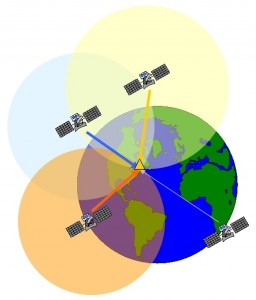
\includegraphics[scale = 0.3]{images/trilateration.jpg}
	\caption{Trilateration using 4 satellites \cite{I1}}
\end{figure}
%\subsection{Subsection Heading Here}
%Subsection text here.


%\subsubsection{Subsubsection Heading Here}
%Subsubsection text here.


% An example of a floating figure using the graphicx package.
% Note that \label must occur AFTER (or within) \caption.
% For figures, \caption should occur after the \includegraphics.
% Note that IEEEtran v1.7 and later has special internal code that
% is designed to preserve the operation of \label within \caption
% even when the captionsoff option is in effect. However, because
% of issues like this, it may be the safest practice to put all your
% \label just after \caption rather than within \caption{}.
%
% Reminder: the "draftcls" or "draftclsnofoot", not "draft", class
% option should be used if it is desired that the figures are to be
% displayed while in draft mode.
%
%\begin{figure}[!t]
%\centering
%\includegraphics[width=2.5in]{myfigure}
% where an .eps filename suffix will be assumed under latex, 
% and a .pdf suffix will be assumed for pdflatex; or what has been declared
% via \DeclareGraphicsExtensions.
%\caption{Simulation results for the network.}
%\label{fig_sim}
%\end{figure}

% Note that the IEEE typically puts floats only at the top, even when this
% results in a large percentage of a column being occupied by floats.


% An example of a double column floating figure using two subfigures.
% (The subfig.sty package must be loaded for this to work.)
% The subfigure \label commands are set within each subfloat command,
% and the \label for the overall figure must come after \caption.
% \hfil is used as a separator to get equal spacing.
% Watch out that the combined width of all the subfigures on a 
% line do not exceed the text width or a line break will occur.
%
%\begin{figure*}[!t]
%\centering
%\subfloat[Case I]{\includegraphics[width=2.5in]{box}%
%\label{fig_first_case}}
%\hfil
%\subfloat[Case II]{\includegraphics[width=2.5in]{box}%
%\label{fig_second_case}}
%\caption{Simulation results for the network.}
%\label{fig_sim}
%\end{figure*}
%
% Note that often IEEE papers with subfigures do not employ subfigure
% captions (using the optional argument to \subfloat[]), but instead will
% reference/describe all of them (a), (b), etc., within the main caption.
% Be aware that for subfig.sty to generate the (a), (b), etc., subfigure
% labels, the optional argument to \subfloat must be present. If a
% subcaption is not desired, just leave its contents blank,
% e.g., \subfloat[].


% An example of a floating table. Note that, for IEEE style tables, the
% \caption command should come BEFORE the table and, given that table
% captions serve much like titles, are usually capitalized except for words
% such as a, an, and, as, at, but, by, for, in, nor, of, on, or, the, to
% and up, which are usually not capitalized unless they are the first or
% last word of the caption. Table text will default to \footnotesize as
% the IEEE normally uses this smaller font for tables.
% The \label must come after \caption as always.
%
%\begin{table}[!t]
%% increase table row spacing, adjust to taste
%\renewcommand{\arraystretch}{1.3}
% if using array.sty, it might be a good idea to tweak the value of
% \extrarowheight as needed to properly center the text within the cells
%\caption{An Example of a Table}
%\label{table_example}
%\centering
%% Some packages, such as MDW tools, offer better commands for making tables
%% than the plain LaTeX2e tabular which is used here.
%\begin{tabular}{|c||c|}
%\hline
%One & Two\\
%\hline
%Three & Four\\
%\hline
%\end{tabular}
%\end{table}


% Note that the IEEE does not put floats in the very first column
% - or typically anywhere on the first page for that matter. Also,
% in-text middle ("here") positioning is typically not used, but it
% is allowed and encouraged for Computer Society conferences (but
% not Computer Society journals). Most IEEE journals/conferences use
% top floats exclusively. 
% Note that, LaTeX2e, unlike IEEE journals/conferences, places
% footnotes above bottom floats. This can be corrected via the
% \fnbelowfloat command of the stfloats package.




\section{Assumptions}
\begin{enumerate}
\item Earth's shape is modeled by an ellipsoid which means that geometrically, the equatorial radius is longer than the
polar axis by about 23 km. The direction of gravity does not point to the center of the earth. This model is used to convert the geocentric coordinates of user[X,Y,Z] to the geodetic model and  locate the latitude, longitude and height on the Google maps.
\begin{figure}[h]
	\centering
	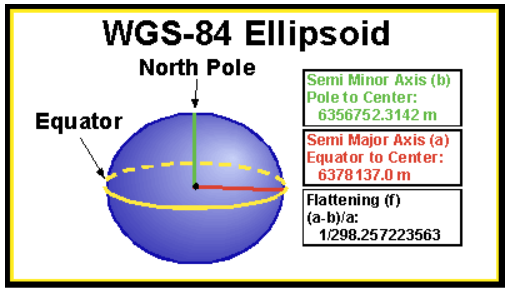
\includegraphics[scale = 0.5]{images/ellipse.png}
	\caption{Earth ellipsoid model\cite{I2}}
\end{figure}
\item In order to get the user position from this algorithm at any instant 4 or more satellites must be visible to the user. The satellite constellation is designed in such a way.
\item Least square solution converges after only 4 or 5 iterations. Which means that the value of "dx" (Difference between the true and calculated position) and "db" (Difference in actual and calculated user clock bias) is reduced to e-3 in these iterations when the corrected pseudo range, user clock bias and errors are fed back in each iteration.
\item The values of constants for GPS equations like c (Speed of light), $\mu$ (Earth's gravitational constant), $\dot{\theta}$ (Earth's rotation rate), F (rel cor term constant). The initial value of $\tau$ = 0.075 sec. This value is updated in each iteration of algorithm.
\end{enumerate}

\section{Flowchart for the matlab code}
Here the flowchart of the matlab main code is explained and in further sections each component of the code is explained specifying how each component is calculated.

% conference papers do not normally have an appendix
\begin{figure}[!h]
	\centering
	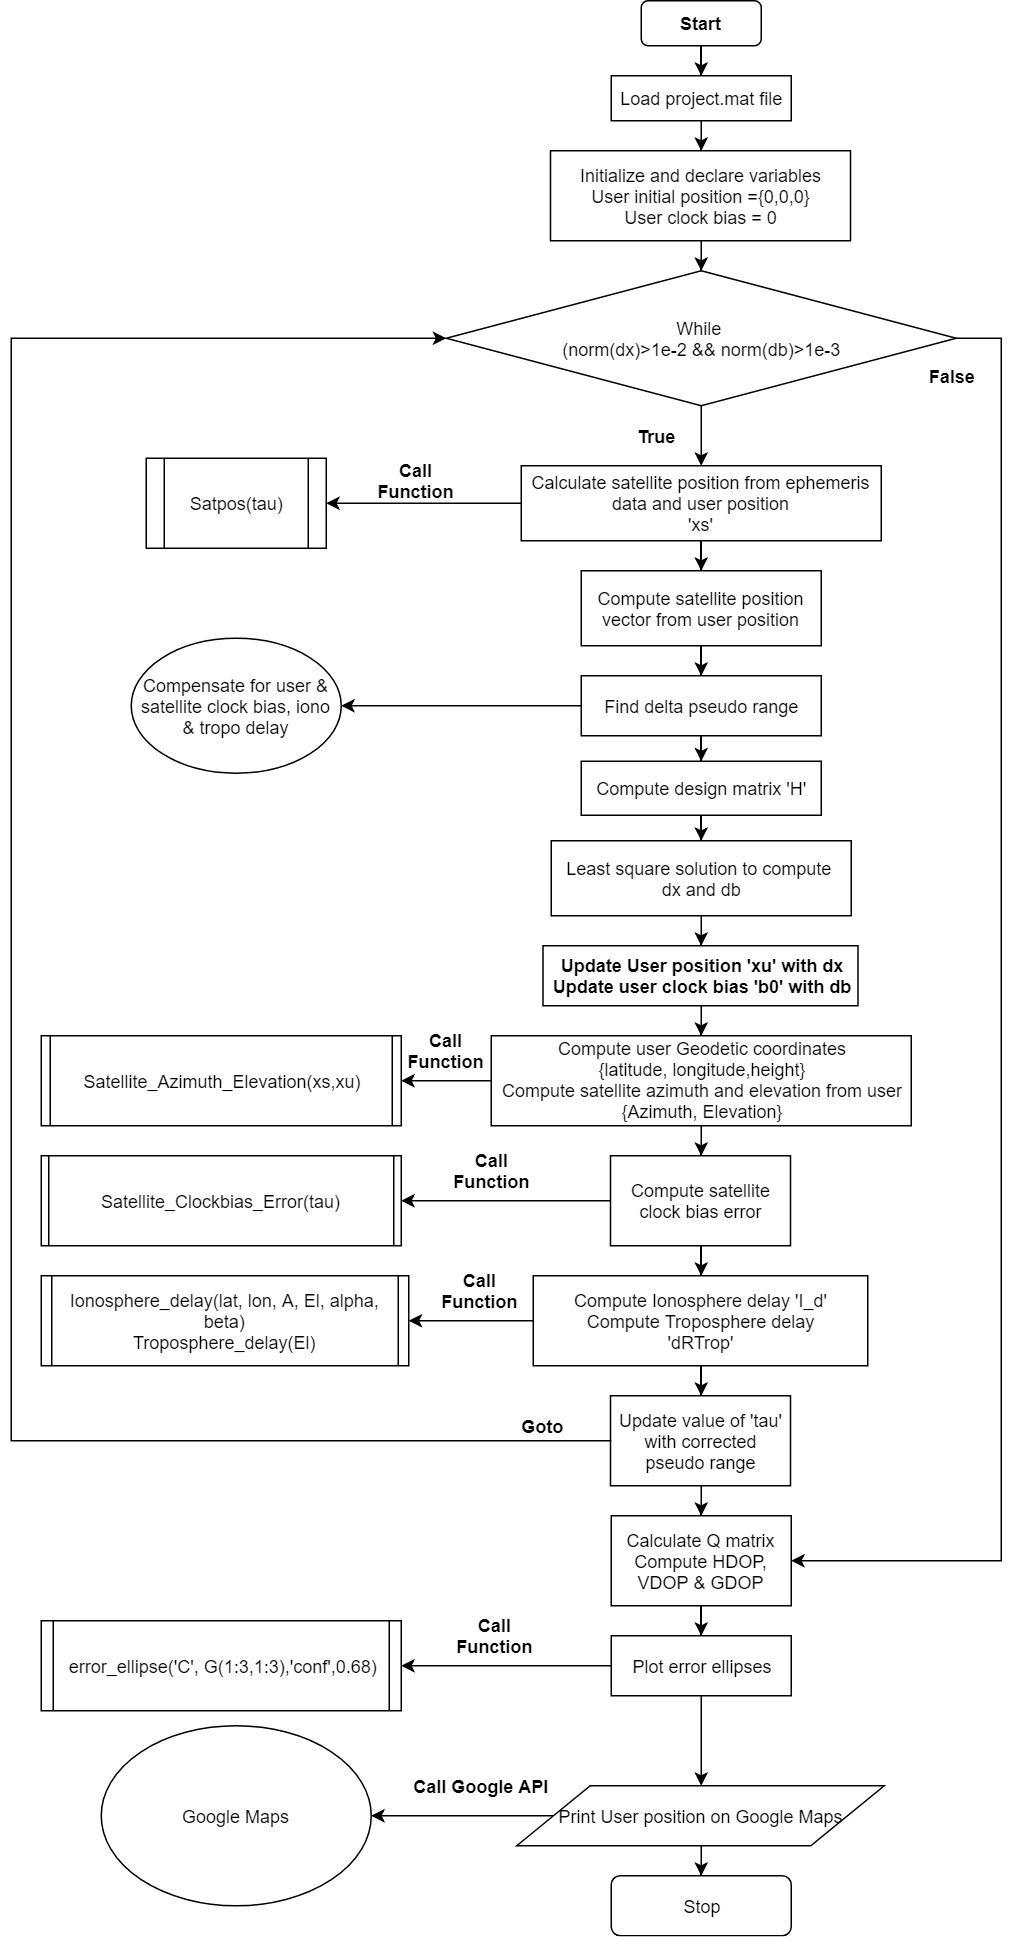
\includegraphics[scale = 0.25]{images/flowchart.jpg}
	\caption{Flowchart for matlab code}
\end{figure}

\section{Components of the code}
\subsection{Ephemeris data from satellites}
Project\_data$\cdot$ mat file consists of ephemeris data from 6 satellites. It also includes values of pseudorange measured by receiver as "pr". Iono error constants as "iono". Theses values are extracted into respective variables. 
\subsection{Initial position of user and user clock bias}
For starting the algorithm initial position of user is geocentric origin of the ECEF coordinate system i.e [0,0,0]. User clock bias is also assumed to be [0].

\subsection{Satellite position from Ephemeris data}
Calculating Satellite position from ephemeris is given in \cite{doc1} i.e IS-GPS-200D. Following images taken from \cite{doc1} tell about the parameters involved in finding coordinates and also the equations for calculation. Output $x^k$, $y^k$, $z^k$ are the ECEF coordinates. "Satpos.m" function does the calculation. The input for this function is $\tau$ which is updated in each iteration.
\begin{figure}[!h]
	\centering
	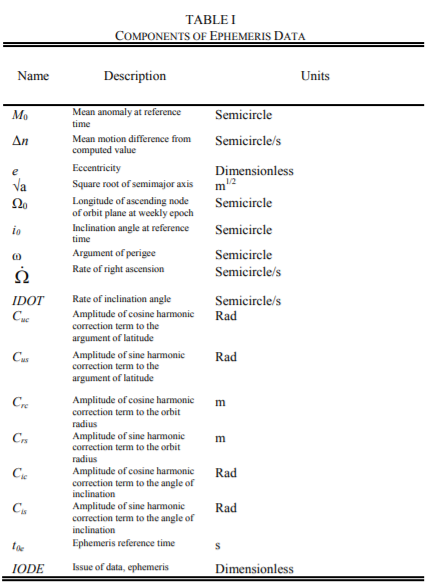
\includegraphics[scale = 0.5]{images/table1.png}
	\caption{}
\end{figure}
\begin{figure}[!h]
	\centering
	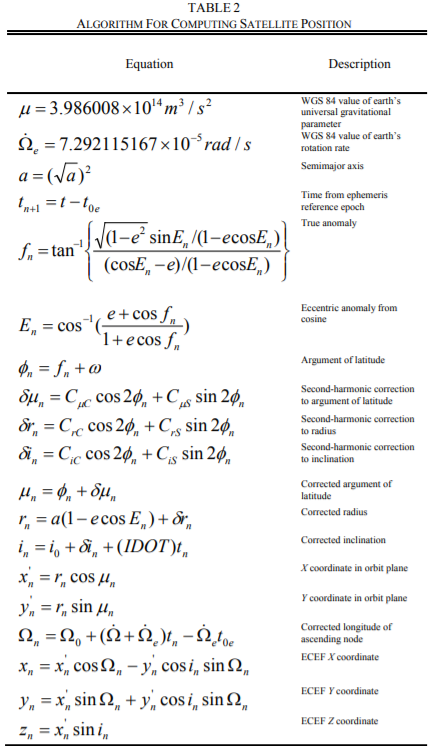
\includegraphics[scale = 0.5]{images/table2.png}
	\caption{}
\end{figure}
\subsection{Compute satellite position vector from user}
Satellite position obtained in the previous step is utilized to find the position vector from user to satellite.
\subsection{Calculate the $\delta\rho$ } 
The equation used to calculate the $\delta\rho$ is mentioned:
\begin{IEEEeqnarray}{rCl}
\delta\rho & = & \rho_{measured} - \rho_{corrected}\\
\rho_{measured} &=& pr \nonumber\\ 
\rho_{corrected} &=& \sqrt{(x^k-x_u)^2 + (y^k-y_u)^2  + (z^k-z_u)^2  }  \nonumber\\ && + (b_0 - c*(\delta T_{clk}^{st})) +  c*I_d + \delta RTrop \nonumber
\end{IEEEeqnarray}
where
\begin{IEEEeqnarray}{rCl}
	xu = x_u, y_u, z_u &=& \textnormal{User's coordinates in ECEF system} \nonumber\\
	xs = x^k, y^k, z^k &=& \textnormal{Satellite's coodinates in ECEF system}\nonumber\\
	b_0 &=& \textnormal{User's clock bias} \nonumber\\
	c &=& \textnormal{Speed of light} \nonumber\\
	\delta T_{clk}^{st} &=& \textnormal{Satellite's clock bias error} \nonumber\\
	I_d &=& \textnormal{Ionosphere delay} \nonumber\\
	\delta RTrop &=& \textnormal{Troposphere delay} \nonumber
\end{IEEEeqnarray}
\subsection{Compute design matrix H } 
\begin{IEEEeqnarray}{rCl}
H = [-\text{Satellites position unit vector} \hfil   \text{ones(1,6)}]_\text{6x4}
\end{IEEEeqnarray}

\subsection{Least square solution}
\begin{IEEEeqnarray}{rCl}
\delta r = (H^T \cdot H)^{-1} \cdot H^T \cdot \delta\rho
\end{IEEEeqnarray}

\subsection{Update user position and user clock bias error}
\begin{IEEEeqnarray}{rCl}
	xu &=& xu + \delta x \nonumber\\
	b_0 &=& b0 + \delta b \nonumber
\end{IEEEeqnarray}
where
\begin{IEEEeqnarray}{rCl}
	\delta x &=& \delta r(1:3)  \nonumber\\
	\delta b &=& \delta r(4)  \nonumber
\end{IEEEeqnarray}


\subsection{Calculate satellite Azimuth and Elevation from user position}
This is calculates by Satellite\_Azimuth\_Elevation function.
The inputs to this function are user and satellite position in ECEF coordinates i.e xu \& xs. Output of this function is satellite Azimuth "A", Elevation "E" in radians and users latitude "lat", longitude "lon" in degrees and height "h" in meters.
This is done in three steps
\begin{enumerate}
	\item Convert users ECEF coordinates to geodetic [lat, lon, h]
	\item Convert the satellites position vector coordinate from user position into ENU coordinate system [E,N,U]
	\item Calculate Azimuth and Elevation
	\begin{IEEEeqnarray}{rCl}
		A &=& \text{atan2(E,N)} \\
		E &=& \text{asin(U/norm[E,N,U])}
	\end{IEEEeqnarray}
\end{enumerate}


\subsection{Calculate clock bias error of satellites}
The function used to calculate this is Satellite\_Clockbias\_Error. Input to this function is "$\tau$" and output is $\delta T_{clk}^{st}$ in seconds.
The equation utilized to calculate is 
\begin{IEEEeqnarray}{rCl}
\delta T_{clk}^{st}  &= & af0 + af1\cdot T + af2\cdot (T)^2 + \nonumber\\ && F\cdot e \cdot sqrtA \cdot sin(Ek)- Tgd
\end{IEEEeqnarray}
 The values of constants is taken from project\_data$\cdot$ mat file. The value of input "$\tau$" is updated in each iteration

\subsection{Calculate Ionosphere delay}
This is done by the Ionosphere\_delay function. There are 6 inputs to this function; user\textquotesingle s latitude (lat), longitude (lon) in degrees and satellite azimuth (A) and elevation (E) in radians, alpha, beta values from iono matrix.
The output of this function is I\_d in seconds.
Klobuchar\textquotesingle s Algorithm \cite{doc2} is utilized to calculate delay.

\subsection{Calculate Troposphere delay}
The Troposphere\_delay function calculates it. The input to this function is the elevation (E) in radians of the satellite from user position. The output of this function is the $\delta$ RTrop in meters. the equation used to calculate is: 
\begin{IEEEeqnarray}{rCl}
\delta RTrop &=& 2.312/sin(\sqrt{E\cdot E+1.904e-3}) + \nonumber \\ && 0.084/sin(\sqrt{E\cdot E + 0.6854e-3})
\end{IEEEeqnarray}

\subsection{Update value of $\tau$ for next iteration}
 \begin{IEEEeqnarray}{rCl}
\tau_{new} = \tau_{old}+ \delta\rho/c 
 \end{IEEEeqnarray}
 For each iteration a new value of $\tau$ is calculated which is passed to all the depending functions.
 
 \section{Results}
 \begin{enumerate}
 	\item The iteration runs for 5 times to reduce the value of $\delta$x and $\delta$b to the required threshold.
 	\item The final coordinates of the receiver in ECEF system are :
 	\begin{IEEEeqnarray}{rCl}
 		x &=& 3.8952*1.0e+06 \nonumber\\
 		y &=& 0.3147*1.0e+06\nonumber\\
 		z &=& 5.0241*1.0e+06\nonumber
 	\end{IEEEeqnarray}
 	and in geodetic system i.e [lat,lon,h] are:
 	\begin{IEEEeqnarray}{rCl}
 		lat &=& 52.3093\, \degree N \nonumber\\
 		lon &=& 4.6197 \,\degree E\nonumber\\
 		h &=& 197.7866\, m\nonumber
 	\end{IEEEeqnarray}
    \item These coordinates are plotted on Google maps
    as shown below by a \textcolor{red}{red} point:
    \begin{figure}[!h]
    	\centering
    	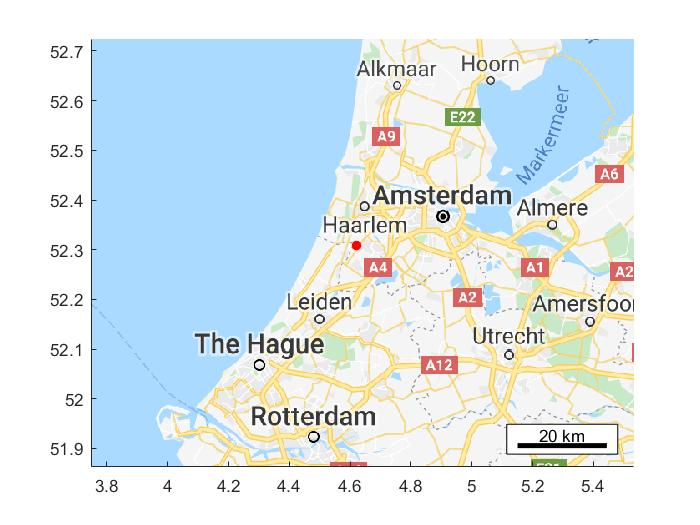
\includegraphics[scale = 0.3]{images/final_location.jpg}
    	\caption{   Final location on map}
    \end{figure}
 \end{enumerate}
 
 \section{Error Analysis}
 \begin{enumerate}
 	\item  Covariance matrix is calculated as follows:
 	\begin{IEEEeqnarray}{rCl}
 		G = (H^T\cdot H)^{-1}
 	\end{IEEEeqnarray}
 		G =    
 		$\begin{Bmatrix}
 			10.3175  &  2.1986 &   4.7947   & 8.1054\\
 			2.1986 &   0.9658  &  1.1574  &  1.8529\\
 			4.7947  &  1.1574   & 3.7528  &  4.3210\\
 			8.1054  &  1.8529 &   4.3210  &  6.7478
 		\end{Bmatrix}$\\
 	
 
\item The values of DOP are also acceptable as calculated using formulas below:
\begin{IEEEeqnarray}{rCl}
	HDOP &=& \sqrt{G(1,1)+G(2,2)} = 3.3591 \nonumber\\
	VDOP &=& \sqrt{G(3,3)} = 1.9372 \nonumber\\
	TDOP &=& \sqrt{G(4,4)} = 2.5977 \nonumber\\
	PDOP &=& \sqrt{G(1,1)+G(2,2)+G(3,3)} = 3.8776 \nonumber\\
	GDOP &=& \sqrt{G(1,1)+G(2,2)+G(3,3)+G(4,4)}\nonumber\\& = & 4.6673 \nonumber
\end{IEEEeqnarray}
\item 1-sigma (68.3\%)Error ellipses are plotted using the error\_ellipse \cite{doc3} function. Plots are given below:
\begin{figure}[!h]
	\centering
	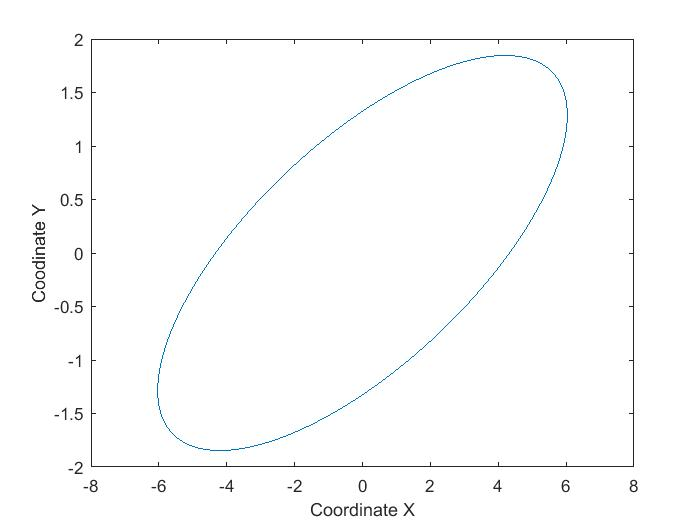
\includegraphics[scale = 0.15]{images/xy.jpg}
	\caption{X-Y coordinate variance}
\end{figure}
\begin{figure}[!h]
	\centering
	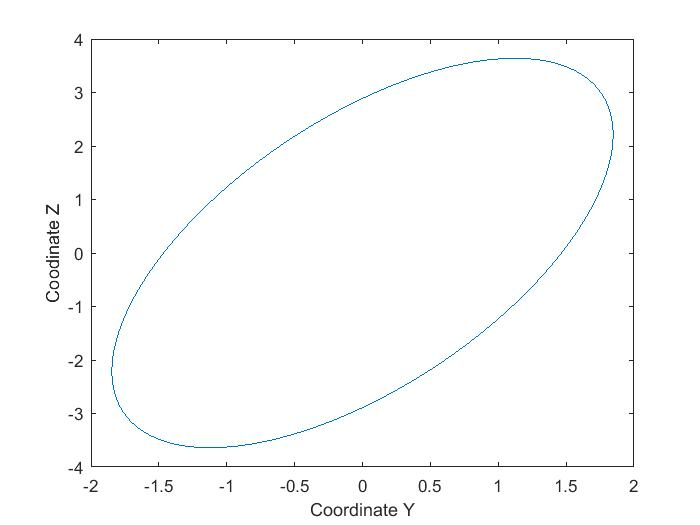
\includegraphics[scale = 0.15]{images/yz.jpg}
	\caption{Y-Z coordinate variance}
\end{figure}
\begin{figure}[!h]
	\centering
	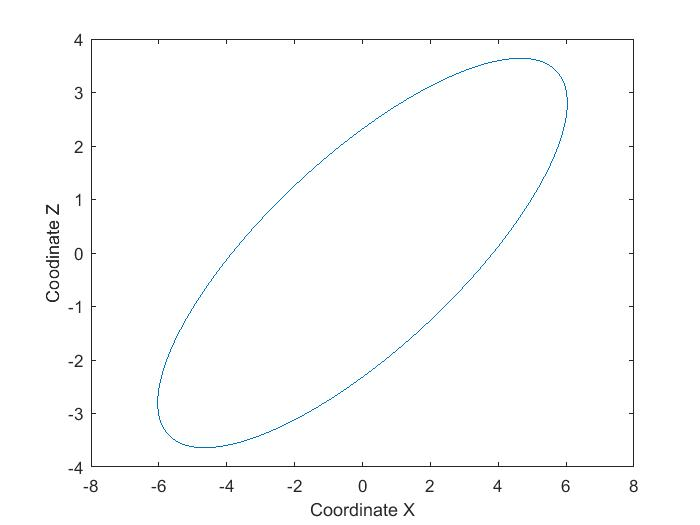
\includegraphics[scale = 0.15]{images/xz.jpg}
	\caption{X-Z coordinate variance}
\end{figure}
\end{enumerate}

\section{Conclusion}
The ephemeris data received from satellites was utilized to calculate the satellite position, satellite clock bias error, ionosphere delay, troposphere delay and then using pseudorange equation and least square solution user coordinates and user clock bias was calculated. GPS user location was ploted on Google maps using Google API. Error analysis was successfully carried out using dilution of precision and error ellipses. The values of DOP were also acceptable.
The MATLAB code has been added in the appendix.
% trigger a \newpage just before the given reference
% number - used to balance the columns on the last page
% adjust value as needed - may need to be readjusted if
% the document is modified later
%\IEEEtriggeratref{8}
% The "triggered" command can be changed if desired:
%\IEEEtriggercmd{\enlargethispage{-5in}}

% references section

% can use a bibliography generated by BibTeX as a .bbl file
% BibTeX documentation can be easily obtained at:
% http://mirror.ctan.org/biblio/bibtex/contrib/doc/
% The IEEEtran BibTeX style support page is at:
% http://www.michaelshell.org/tex/ieeetran/bibtex/
%\bibliographystyle{IEEEtran}
% argument is your BibTeX string definitions and bibliography database(s)
%\bibliography{IEEEabrv,../bib/paper}
%
% <OR> manually copy in the resultant .bbl file
% set second argument of \begin to the number of references
% (used to reserve space for the reference number labels box)
\begin{thebibliography}{1}
\bibitem{I1}
https://www.sxbluegps.com/technology/gps-the-error-budget/
\bibitem{I2}
https://www.unavco.org/education/resources/tutorials-and-handouts/tutorials/elevation-and-geoid.html
\bibitem{doc1}
https://www.navcen.uscg.gov/pdf/IS-GPS-200D.pdf
\bibitem{doc2}
\url{https://gssc.esa.int/navipedia/index.php/Klobuchar_Ionospheric_Model}
\bibitem{doc3}
\url{https://www.mathworks.com/matlabcentral/fileexchange/4705-error_ellipse}

\end{thebibliography}




% that's all folks
\end{document}


